\chapter{Data gathering implementation}
\label{ch:gathering}
As mentioned before in this thesis, the \textit{data\_gathering} container consists of a Python project, which main function is to collect card market data. Static data is acquired once, dynamic data daily, and the validity of the data is ensured after every run. The user can alter the program's operation by changing values in the configuration file, and the responses are provided in console and log files. The core part of the implementation in contained in \textit{web} and \textit{data} services. After this container completes its objective, the CSV files in data directory are updated with the newest information available, and their checksum is calculated to be retained as a marker for the verified dataset.


\section{Program configuration}
The configurable global variables are stored in file \textit{config.py}. There are three subgroups inside:

\begin{enumerate}
      \item Variables for user custom program configuration. \par
            \texttt{START\_FROM = 1\\ FORCE\_UPDATE = False\\ EXPANSION\_NAME = `Battlebond'} \par
            The user may want to renew the daily data when suspecting incompleteness or start the operation from a specific card id (for example, starting from 128 when the previous run crashed after card 127). Moreover, the user is provided with the ability to change the expansion, so that efectively all cards from the game could be gathered.
      \item Variables connected to a single run of code. \par
            \texttt{DATE\_ID = 0\\ MAIN\_LOGNAME = `other\_main.log'\\ RUN\_LOGNAME = `other\_run.log'} \par
            These values are determined at the start of the run (whenever a new date has been detected). Log filenames are unique to the run and are used by the logging service. Shared date id is crucial for all operations of the program.
      \item Fixed variables. \par
            \texttt{CONTAINER\_DELAY = 10\\ NAME = `data-gathering'\\ BASE\_URL = `https://www.cardmarket.com/en/Magic/Products/Singles/'\\ USERS\_URL = `https://www.cardmarket.com/en/Magic/Users/'\\ WEBDRIVER\_HOSTNAME = `firefox\_webdriver'\\ HEADERS = \textbraceleft"date": \textbraceleft"id": "int", "day": "int", \dots\textbraceright, "card": \dots\textbraceright} \par
            Fixed variables are used for internal program logic. They are aggregated in a single file to be changed with convenience and to be available wherever needed by importing the file. They set up the website's paths, connection details and information about entities columns and data types.
\end{enumerate}

\section{Used services}
\label{s:used_services}
The program uses four services:
\begin{itemize}
      \item \textit{Web service}.
            Responsible for handling the connection to the remote webdriver in another container. It serves as an interface for acquiring the cards' names from specified expansion; loading card and seller pages; clicking the \textit{Load more} button to expand the page fully; getting website's source code in form of a Beautiful Soup object; cooling the connection down to prevent HTML response status 429\footnote{Too  Many Requests --- The user has sent too many requests in a given amount of time ("rate limiting").}; and verifying the completeness of loaded pages.

      \item \textit{Data service}.
            This biggest singular service (over 700 lines of code) utilizes the \textit{Pandas} library to take apart soup objects and transform the information they hold into data records in csv files. This module also provides quasi-database-like functionalities, like finding card's id by its name or checking whether a particular sellers or card statistics are already saved. Here one can also find the use of \textit{pickle} data format, which is astonishingly fast in comparison with other data extensions, as well as the logic responsible for pickling, unpickling, updating and verifying the data.

      \item \textit{Flags service}.
            The main use for this service in \textit{data\_gathering} container is to signal whenever a dataset has been checked (collected data is tested against various inconsistencies, for example the number of card statistics from each day should equal the number of cards, etc). When the data appears to be complete, the checksum of the entire data directory is calculated and saved in a shared file, for the next stages of the data pipeline to access and confront the datasets against.

      \item \textit{Logs service}.
            This simple service is a wrapper for the print command. It uses the current time and values from the configuration file to display the state of the program in the console and generated log file. Each container generates a log subdirectory for its own purpose.
\end{itemize}

To keep the operation of the program simple and fast the author decided to prefer modular programming over object-oriented programming. OOP approach would probably yield some simplicity with methods related to the entities (e.g. \textit{Card} class, with scraping the data, importing, exporting and updating inside the class body as methods), but it would entail sharing the class among containers, which would require all of the containers to have the same external libraries installed, which would reduce their build time and performance. Using functions on module-levels, with separation of resposibility between modules ensures minimal redundancy in importing external libraries, as well as provides fast and readable code.


\section{Local directories}
The container is given access to three host directories via bind mounts: \textbf{data}, where the csv files are stores; \textbf{logs}, with data-gathering subdirectory filled with daily and run-level logs; and \textbf{flags}, containing SHA-1 formatted file with a list of checksums of verified datasets. \par
There is also a docker volume named \textit{pickle\_data}, which maps to a folder named \textbf{.pickles} in the container root directory. This space is a storage for the data in pickle format, used only by that container during a gathering run.

\section{Run scheduling}
The program begins by booting the directories up if they don't exist and determining the current date. If it's not added to \textit{date.csv}, new entry in the file is generated and its date id is returned. Otherwise, just the date id is retrieved from an existing date. Then, the execution is halted inside a scheduling loop, until the conditions for running the gathering procedure are met. \par \noindent
\texttt{\# Setup \\ logs.setup\_logs() \\ data.setup\_data() \\ flags.setup\_flags() \\ data.add\_date() \\ \\ \# Time the program execution \\ data.schedule\_the\_run()}

As seen on Fig. \ref{fig:gathering_schedule}, the run scheduling function checks whether the configuration flag \linebreak \texttt{config.FORCE\_UPDATE} is set or whether it's a first gathering run in the environment, which results in immediate return of control to the main function. \par
If that's not the case, the data directory checksum gets calculated and compared to the validated hashes. In case of occurence in the control file, the program sleeps for 60 minutes, as current data has been validated to be complete. When there is no entry in the \textit{validated\_checksums.sha1} file, the program checks whether today's data is complete. If not, the operation proceedes to gather the data, otherwise it saves the checksum as verified and waits 60 minutes. Every time after sleeping, the date is checked and date id is chosen accordingly.

\begin{figure}[ht]
      \centering
      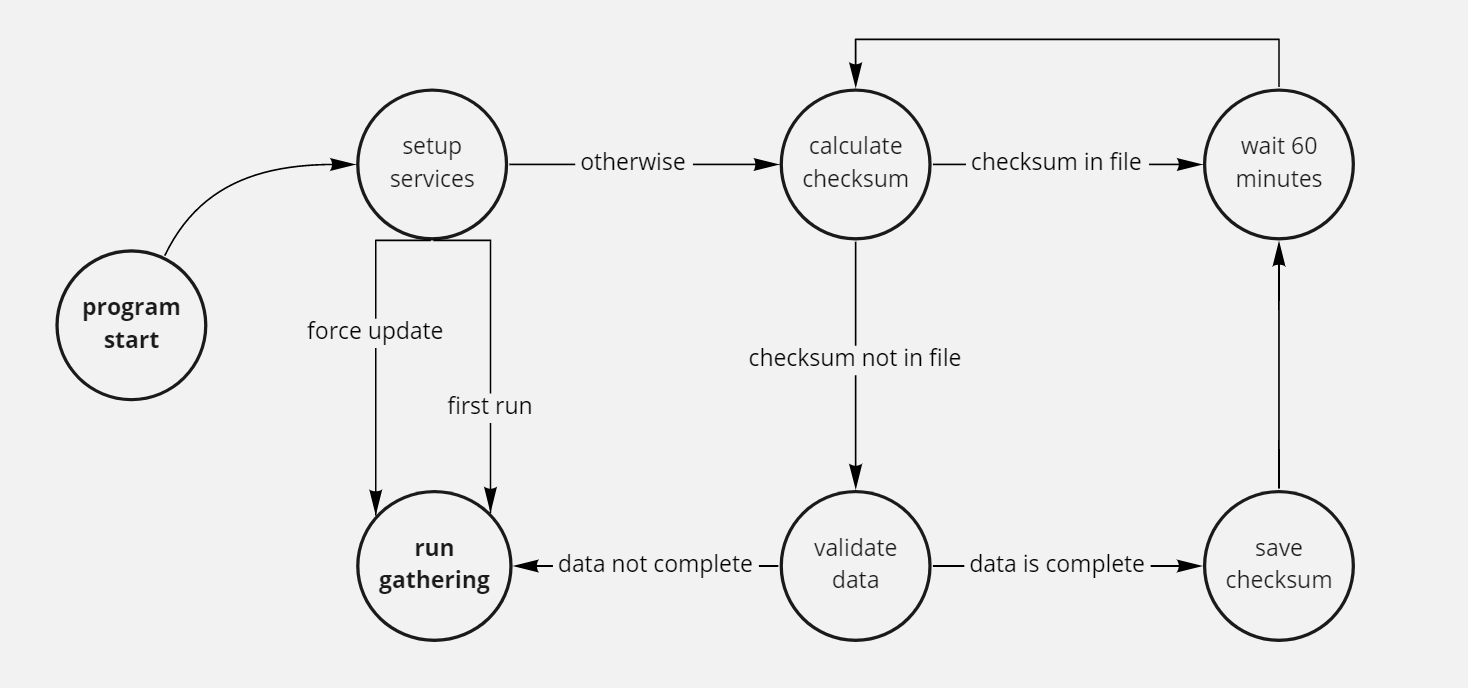
\includegraphics[width=\textwidth]{figures/gathering_schedule.png}
      \caption{Program states in data gathering scheduling}
      \label{fig:gathering_schedule}
\end{figure}

\section{Data pickling and validation}
Initially the data was stored in raw csv files, with each new entry being appended to the end as text. This approach proved to be conceptually simple, but not very scalable, as it yielded higher and higher wait times for opening and closing files with hundreds of thousands of rows. Currently, the \textit{sale\_offer.csv} file stores roughly 10 million rows of data, but the total waiting time for opening, reading, writing and closing is greatly reduced. This is done by using the pickle data format with very fast r/w speed. Between the runs, data is kept in gzip-compressed csv format, to ensure minimal disk usage. However, as the run begins, some of the files are read into dataframes and converted to intermediate \textit{.pkl} files. Then, whenever a pickled entity is needed, the program knows to read the pickle file instead, which loads about 100 times faster. When the program is finished, the pickled entities are transformed back to csv format. This step is the biggest hazard of potential data loss, as hours of computation kept in few, hidden files replace the previous data in a matter of minutes. \par
The pickle data format posed another challenge: unexpected errors concerning pickling directories and iteratively growing a pickle object. Unfortunately, the approach to acquiring sellers and cards was exactly that; a dictionary with pairs of attirbutes and values represents a single seller and to keep all entries, a list is used. Unpickling the whole object to add one seller and then pickle it back was causing the data to become unreadable after few hundret iterations. The speed of operating on gzip-compressed CSV files with less than 10 thousand rows was acceptable, especially taking into account that sellers are only added when they are not in the table, but sale offers and card stats are updated every day. \par

\begin{figure}[ht]
      \centering
      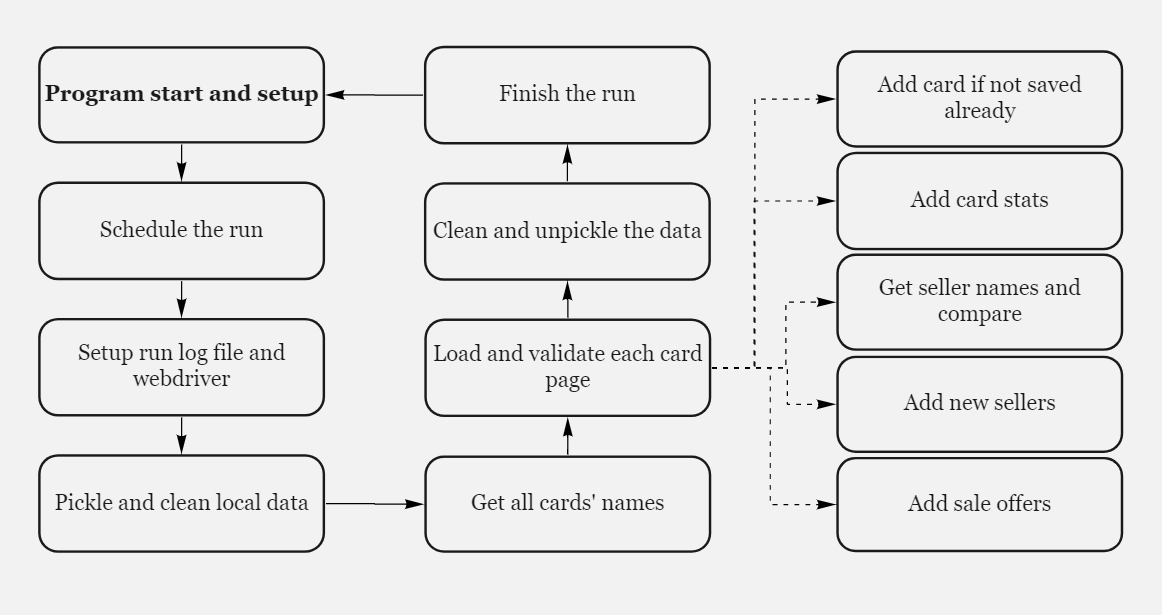
\includegraphics[width=\textwidth]{figures/gathering_flow.png}
      \caption{Program states in data gathering scheduling}
      \label{fig:gathering_flow}
\end{figure}

\section{Loop over cards}
The program works by querying the local TXT file with names of the cards and creating proper card urls according to a template. The webdriver loads the page with explicit wait time equal to 1.5 seconds, which gives this much time for the request elements to load. The card page features all the card information and a list of sale offers which can be expanded by clicking a ``Load more'' button on the bottom of the page. This button is one of the reasons for the use of Selenium framework as opposed to \textit{requests}. We need dynamic control of the webpage to interact with the button, until all the offers are loaded. After each click, the program waits up to 1.5 seconds. \par Getting this page is the most network-heavy operation of the code, thus we save the complete webpage as a soup object to be deconstructed later. Each card soup is passed to appropriate methods to extract the card statis information and statistics, as well as the list of offers. After the card processing is completed, a \texttt{START\_FROM} counter is incremented, so that the program can pick up from the last completed task (provided it doesn't fail into restart). After all card pages have been visited, acquired and processed, we clean and unpickle the data, then the program control comes back to the scheduler, where the data can be checked for completness and validated. (IMAGE CARD PAGE)

\section{Soup decomposition}
The card page source, packed in a soup format, is used to get the name of the card. If no such card exists in our records, it is added, together with (IMAGE LOGS ADD NEW CARD) the expansion name, rarity and a unique id. The time-related card characteristics are acquired every time. They need to be updated daily and the most recent data has priority. In case of second run of the day the saved card stats are dropped.
(IMAGE CARD STATS)

\subsection{Sale offers table}
(IMAGE TABLE SALE OFFERS)
Understanding the table of sale offers.

A list of sellers names if acquuired from the source code of the page, along with the list of prices, card conditions and other sale-related information. The seller names are stored in a set, from which we substract all the names of already known sellers. The remaining names are to be saved, so appropriate user page URLs are generated according to a template. Then, every new seller page is visited and data about them is saved to the seller collection. (IMAGE SELLER PAGE) Due to sellers being added cumulatively into the dataframe (use of \texttt{append(seller: dict)}) caused pickles-related fiasco. \par
Updating sale offers is possible because the separate lists of seller names, prices, conditions and other, can be zipped into a dictionary. This way, we're scanning the table vertically and concatenating the attributes together to form a new set of records to be added to the sale offers file. If the offers are already saved that day, the old ones are dropped in favor of the new ones. Complete update however, happend only at the end of the run, when the pickled data is used to replace the pre-run data.


\section{Data pipeline output}
When the program is finished we have a complete list of card names, separate CSV file of static cards information with their IDs. The file with card statistics will have 264 new entries corresponding to each card and any new sellers will be saved in their CSV file. The sale offers file is going to have about 90000 more entries, representing the offers placed by sellers for each card. All the data is stored in five compressed CSV files and one TXT file. The data is ready to be checked for completion (e.g. to detect 263 cards gathered instead of 264). When the data is verified to be complete, a checksum of the data directory is calculated and saved in the validated-checksums.md5 file, so that other containers can recognize this dataset as ready to be pushed forward the data pipeline.
